% -*- program: xelatex -*-
%!TEX TS-program = xelatex
%!TEX encoding = UTF-8 Unicode
% Awesome CV LaTeX Template for CV/Resume
%
% This template has been downloaded from:
% https://github.com/posquit0/Awesome-CV
%
% Author:
% Claud D. Park <posquit0.bj@gmail.com>
% http://www.posquit0.com
%
% Template license:
% CC BY-SA 4.0 (https://creativecommons.org/licenses/by-sa/4.0/)
%


%-------------------------------------------------------------------------------
% CONFIGURATIONS
%-------------------------------------------------------------------------------
% A4 paper size by default, use 'letterpaper' for US letter
\documentclass[11pt, a4paper]{awesome-cv}

% Configure page margins with geometry
\geometry{left=1.4cm, top=.8cm, right=1.4cm, bottom=1.8cm, footskip=.5cm}

% Specify the location of the included fonts
\fontdir[fonts/]

% Color for highlights
% Awesome Colors: awesome-emerald, awesome-skyblue, awesome-red, awesome-pink, awesome-orange
%                 awesome-nephritis, awesome-concrete, awesome-darknight
\colorlet{awesome}{awesome-red}
% Uncomment if you would like to specify your own color
% \definecolor{awesome}{HTML}{CA63A8}

% Colors for text
% Uncomment if you would like to specify your own color
% \definecolor{darktext}{HTML}{414141}
% \definecolor{text}{HTML}{333333}
% \definecolor{graytext}{HTML}{5D5D5D}
% \definecolor{lighttext}{HTML}{999999}

\usepackage{kotex}
\usepackage{xifthen}		% To support optional argument for newcommand
\usepackage{hyperref}		% To support hyperlink for newcommand
\usepackage{mfirstuc}

\setmainhangulfont{NanumGothic}
\setsanshangulfont{NanumGothic}

% Set false if you don't want to highlight section with awesome color
\setbool{acvSectionColorHighlight}{true}

% If you would like to change the social information separator from a pipe (|) to something else
\renewcommand{\acvHeaderSocialSep}{\quad\textbar\quad}


%-------------------------------------------------------------------------------
%	PERSONAL INFORMATION
%	Comment any of the lines below if they are not required
%-------------------------------------------------------------------------------
\name{Jonghoon}{Seo}
\position{Software Engineer{\enskip\cdotp\enskip}Doctor of Philosophy in Computer Science}
\address{8, Yeonmujang 11-gil, Seongdong-gu, Seoul, Rep. of Korea}

\mobile{(+82) 10-8357-1688}
\email{jonghoon.seo@gmail.com}
% \homepage{www.posquit0.com}
\github{jonghoonseo}
\linkedin{jonghoonseo}
% \stackoverflow{SO-id}{SO-name}
% \twitter{@jonghoonseo}
% \skype{skype-id}
% \reddit{reddit-id}
% \extrainfo{extra informations}

% \quote{``Must be the change that you want to see in the world."}

%-------------------------------------------------------------------------------
%	BIBLIOGRAPHY
%-------------------------------------------------------------------------------
\addbibresource{cv/resources/my_publications.bib}

%-------------------------------------------------------------------------------
\begin{document}

% Print the header with above personal informations
\makecvheader

% Print the footer with 3 arguments(<left>, <center>, <right>)
% Leave any of these blank if they are not needed
\makecvfooter
  {\today}
  {Jonghoon Seo~~~·~~~Curriculum Vitae}
  {\thepage}


%-------------------------------------------------------------------------------
%	CV/RESUME CONTENT
%	Each section is imported separately, open each file in turn to modify content
%-------------------------------------------------------------------------------
%!TEX root = ../cv.tex
% -*- root: ../cv.tex -*-

%-------------------------------------------------------------------------------
% SECTION TITLE
%-------------------------------------------------------------------------------
\cvsection{Education}


%-------------------------------------------------------------------------------
% CONTENT
%-------------------------------------------------------------------------------
\begin{cventries}

%---------------------------------------------------------
  \cventry
    {컴퓨터정보산업공학과 공학사} % Degree
    {연세대학교} % Institution
    {서울특별시} % Location
    {2001.03 - 2006.02} % Date(s)
    {}

%---------------------------------------------------------

  \cventry
    {컴퓨터과학과 공학석사} % Degree
    {연세대학교} % Institution
    {서울특별시} % Location
    {2006.03 - 2008.02} % Date(s)
    {
      % \begin{cvitems} % Description(s) bullet points
      %   \item {Got a Chun Shin-Il Scholarship which is given to promising students in CSE Dept.}
      % \end{cvitems}
    }

  \cventry
    {컴퓨터과학과 공학박사} % Degree
    {연세대학교} % Institution
    {서울특별시} % Location
    {2008.03 - 2016.08} % Date(s)
    {
      % \begin{cvitems} % Description(s) bullet points
      %   \item {Got a Chun Shin-Il Scholarship which is given to promising students in CSE Dept.}
      % \end{cvitems}
    }
\end{cventries}

%!TEX root = ../cv.tex
% -*- root: ../cv.tex -*-

%-------------------------------------------------------------------------------
% SECTION TITLE
%-------------------------------------------------------------------------------
\cvsection{Work}


%-------------------------------------------------------------------------------
% CONTENT
%-------------------------------------------------------------------------------
\begin{cventries}

%---------------------------------------------------------
  \cventry
    {소프트웨어 엔지니어} % Degree
    {스켈터랩스} % Institution
    {서울특별시} % Location
    {2018.05 - 현재} % Date(s)
    {
      \begin{cvitems} % Description(s) bullet points
        \item {딥러닝 기반 \textbf{결함 검출 시스템 개발})
        \item {결함 객체 검출 모델 개발}
        \item {결함 영역 개선을 위한 전처리 알고리즘 개발}
      \end{cvitems}
    }

%---------------------------------------------------------
  \cventry
    {선임연구원} % Degree
    {LG 전자 전자기술원 인공지능연구소} % Institution
    {서울특별시} % Location
    {2015.03 - 2018.04} % Date(s)
    {
      \begin{cvitems} % Description(s) bullet points
        \item {컴퓨터 비전 기술 기반 \textbf{운전자 상태 인식} 기술 개발}
        \item {\textbf{Qt/QML} 기반 webOS 런처 및 \textbf{그래픽스 컴포지터} 개발}
      \end{cvitems}
    }

%---------------------------------------------------------

  \cventry
    {연구원} % Degree
    {연세대학교 컴퓨터과학과 미디어시스템연구실 (지도교수: 한탁돈)} % Institution
    {서울특별시} % Location
    {2006.03 - 2015.02} % Date(s)
    {
      \begin{cvitems} % Description(s) bullet points
        \item {증강현실 및 손 기반 상호작용 등 차세대 상호작용 기술을 위한 \textbf{컴퓨터 비전 알고리즘} 연구/개발}
        \item {멀티 모달 인터페이스들을 통합하는 상호작용 프레임워크 개발}
        \item {차세대 상호작용 기술을 이용한 UX 설계}
      \end{cvitems}
    }

\end{cventries}

%!TEX root = ../cv.tex
% -*- root: ../cv.tex -*-

%-------------------------------------------------------------------------------
%	SECTION TITLE
%-------------------------------------------------------------------------------
\cvsection{Experience}


%-------------------------------------------------------------------------------
%	CONTENT
%-------------------------------------------------------------------------------
\begin{cventries}
%---------------------------------------------------------
  \cventry
    {Deep Learning} % Job title
    {} % Organization
    {} % Location
    {Level: B+} % Date(s)
    {
      \begin{cvitems} % Description(s) of tasks/responsibilities
        \item {Research on Deep Learning based Object Detection for Defect Detection/Inspection}
        \item {Develop on Steering Wheel Classification Algorithm}
      \end{cvitems}
    }

%---------------------------------------------------------
  \cventry
    {Computer Vision and Pattern Recognition} % Job title
    {} % Organization
    {} % Location
    {Level: B+} % Date(s)
    {
      \begin{cvitems} % Description(s) of tasks/responsibilities
        \item {Develop for Mobile Augmented Reality using Local Feature Tracking \\
               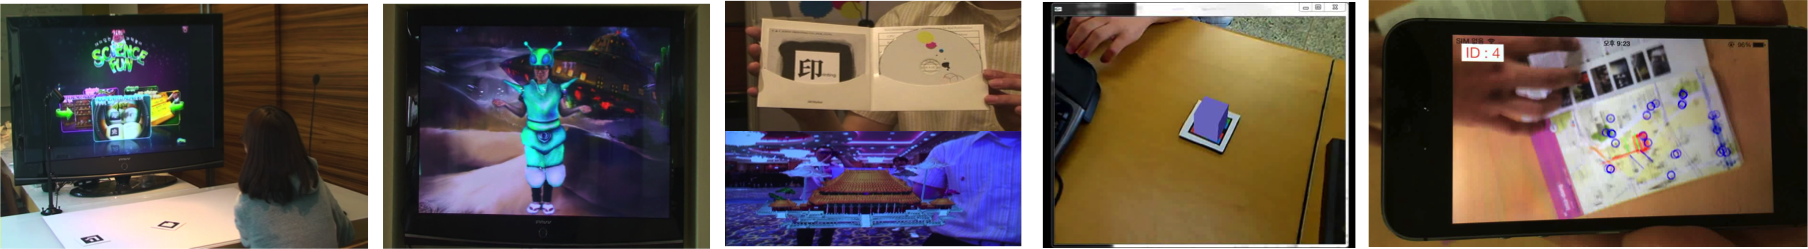
\includegraphics[width=\linewidth]{resources/ar.png} }
          \begin{itemize}
            \item {Develop a feature point filtering algorithm for high performance and speed}
          \end{itemize}
        \item {Research on Recognizing Bare Hands using Depth Camera \\
               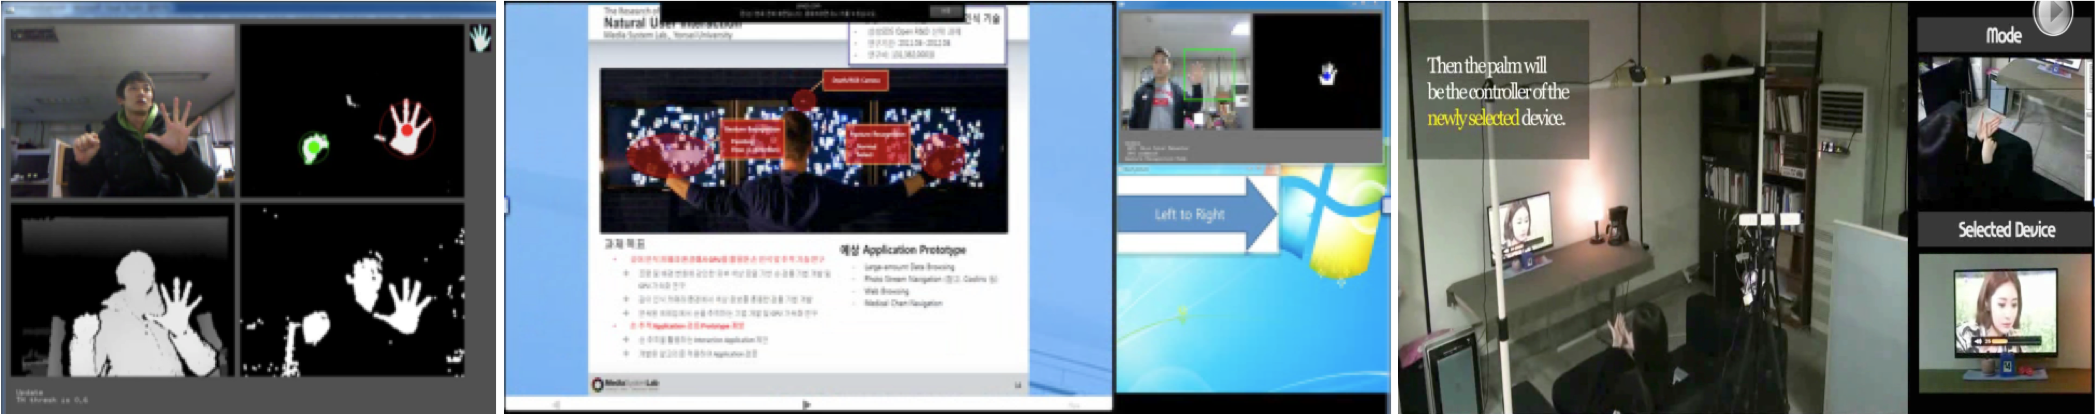
\includegraphics[width=\linewidth]{resources/hand.png} }
        \item {Spoke/Steering Wheel Region Tracking for Driver Status Monitoring}
      \end{cvitems}
    }

%---------------------------------------------------------
  \cventry
    {Device Fast Prototyping} % Job title
    {} % Organization
    {} % Location
    {Level: A+} % Date(s)
    {
      \begin{cvitems} % Description(s) of tasks/responsibilities
        \item {Developing Spatial AR Environment using $360^{\circ}$ Steerable Projector \\
          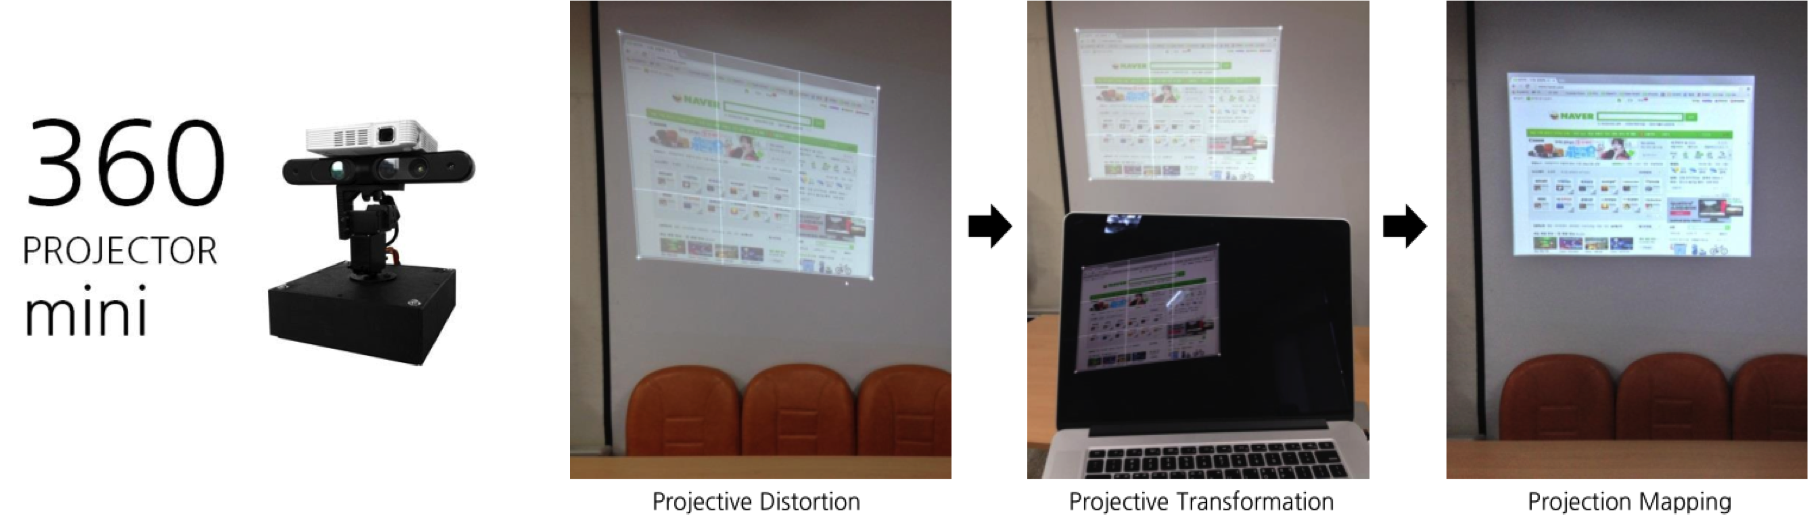
\includegraphics[width=\linewidth]{resources/pervasiveAR.png}
          \begin{itemize}
              \item {Pico Projector, Small Depth Camera, Arduino based Pan-Tilt Motor System}
              \item {Research a computer vision based projecting image rectification algorithm for pan-tilt projector}
          \end{itemize}
        }
        \item {Pen-type Interface which Augments Information on the Surface \\
          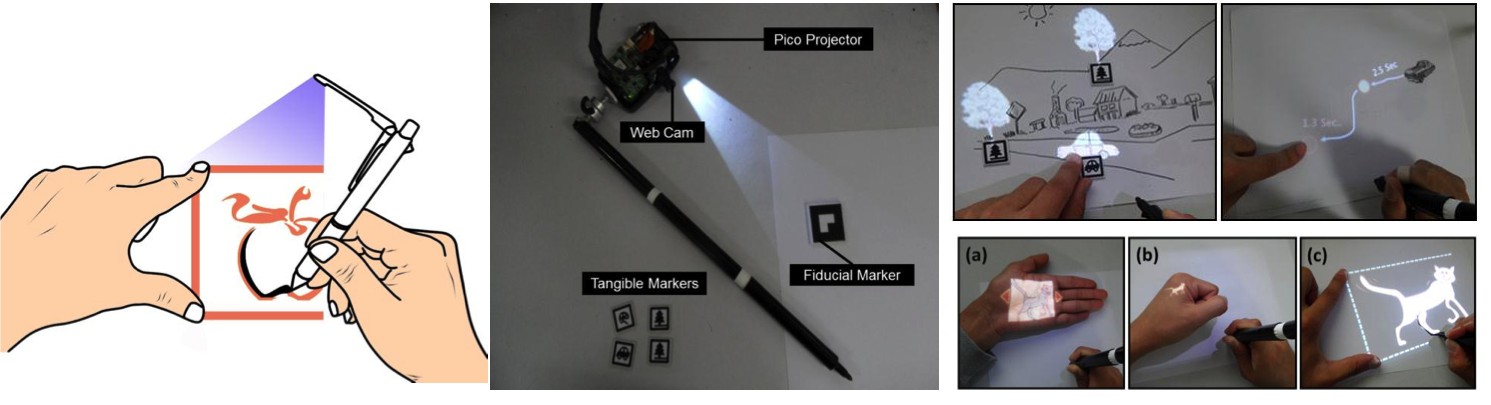
\includegraphics[width=\linewidth, height=40mm]{resources/augpen.png}
          \begin{itemize}
            \item {Pico Projector, Small Web Camera, Fiducial Marker}
            \item {Research on Interating Technology with 2D Contents and Bare Hand}
          \end{itemize}
        }
        \item {Sensor-based Gestural Interfaces \\
          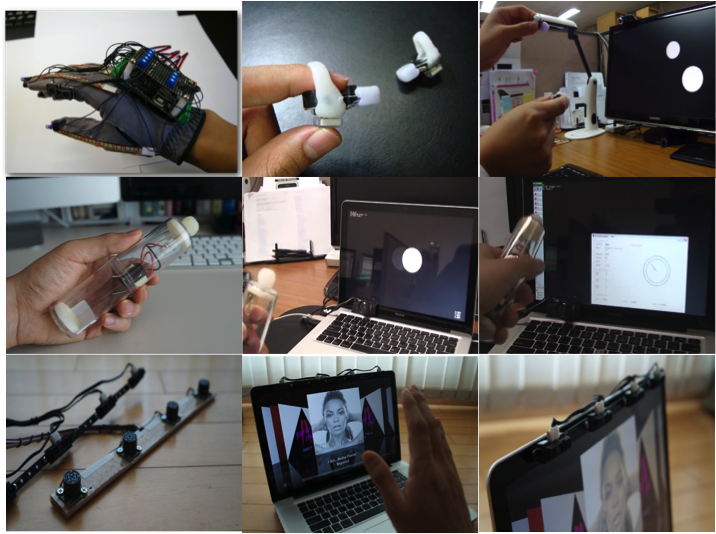
\includegraphics[width=\linewidth]{resources/gesturedevices.png}
          \begin{itemize}
            \item {Developing Various Types of Sensor Interfaces to Recognize Hand Interaction}
            \item {Developing Gesture Interface using IR Blob, Flex Sensor, Gyro Sensor, Lidar Sensor, etc}
          \end{itemize}
        }
      \end{cvitems}
    }
\end{cventries}

%!TEX root = ../cv.tex
% -*- root: ../cv.tex -*-

%-------------------------------------------------------------------------------
%	SECTION TITLE
%-------------------------------------------------------------------------------
\cvsection{Skills}


%-------------------------------------------------------------------------------
%	CONTENT
%-------------------------------------------------------------------------------
\begin{cvskills}

%---------------------------------------------------------
  \cvskill
    {Deep Learning / Computer Vision} % Category
    {TensorFlow, Keras, OpenCV} % Skills

%---------------------------------------------------------
  \cvskill
    {Programming} % Category
    {C/C++, JAVA, Python, QML, C\#} % Skills

%---------------------------------------------------------
  \cvskill
    {SW Frameworks} % Category
    {Qt/QML, OpenFrameworks, Processing, Arduino, Android, WPF} % Skills

%---------------------------------------------------------
  \cvskill
    {Languages} % Category
    {Korean, English} % Skills

%---------------------------------------------------------
\end{cvskills}

%!TEX root = ../cv.tex
% -*- root: ../cv.tex -*-

%-------------------------------------------------------------------------------
%   SECTION TITLE
%-------------------------------------------------------------------------------
\cvsection{Teaching}


%-------------------------------------------------------------------------------
%   CONTENT
%-------------------------------------------------------------------------------
\begin{cvhonors}
  \cvhonor
    {인간과 컴퓨터 상호작용} % Award
    {연세대학교 컴퓨터과학과} % Event
    {서울특별시} % Location
    {2014.09} % Date(s)

  \cvhonor
    {공학전자계산} % Award
    {연세대학교 공과대학} % Event
    {서울특별시} % Location
    {2008.09} % Date(s)

  \cvhonor
    {C 언어 프로그래밍} % Award
    {YJ 학점은행} % Event
    {서울특별시} % Location
    {2008.03} % Date(s)

\end{cvhonors}

%-------------------------------------------------------------------------------
%	SECTION TITLE
%-------------------------------------------------------------------------------
\cvsection{Honors \& Awards}


%-------------------------------------------------------------------------------
%	SUBSECTION TITLE
%-------------------------------------------------------------------------------
\cvsubsection{International}


%-------------------------------------------------------------------------------
%	CONTENT
%-------------------------------------------------------------------------------
\begin{cvhonors}

%---------------------------------------------------------
  \cvhonor
    {Finalist} % Award
    {DEFCON 26th CTF Hacking Competition World Final} % Event
    {Las Vegas, U.S.A} % Location
    {2018} % Date(s)

%---------------------------------------------------------
  \cvhonor
    {Finalist} % Award
    {DEFCON 25th CTF Hacking Competition World Final} % Event
    {Las Vegas, U.S.A} % Location
    {2017} % Date(s)

%---------------------------------------------------------
  \cvhonor
    {Finalist} % Award
    {DEFCON 22nd CTF Hacking Competition World Final} % Event
    {Las Vegas, U.S.A} % Location
    {2014} % Date(s)

%---------------------------------------------------------
  \cvhonor
    {Finalist} % Award
    {DEFCON 21st CTF Hacking Competition World Final} % Event
    {Las Vegas, U.S.A} % Location
    {2013} % Date(s)

%---------------------------------------------------------
  \cvhonor
    {Finalist} % Award
    {DEFCON 19th CTF Hacking Competition World Final} % Event
    {Las Vegas, U.S.A} % Location
    {2011} % Date(s)

%---------------------------------------------------------
\end{cvhonors}


%-------------------------------------------------------------------------------
%	SUBSECTION TITLE
%-------------------------------------------------------------------------------
\cvsubsection{Domestic}


%-------------------------------------------------------------------------------
%	CONTENT
%-------------------------------------------------------------------------------
\begin{cvhonors}

%---------------------------------------------------------
  \cvhonor
    {3rd Place} % Award
    {WITHCON Hacking Competition Final} % Event
    {Seoul, S.Korea} % Location
    {2015} % Date(s)

%---------------------------------------------------------
  \cvhonor
    {Silver Prize} % Award
    {KISA HDCON Hacking Competition Final} % Event
    {Seoul, S.Korea} % Location
    {2017} % Date(s)

%---------------------------------------------------------
  \cvhonor
    {Silver Prize} % Award
    {KISA HDCON Hacking Competition Final} % Event
    {Seoul, S.Korea} % Location
    {2013} % Date(s)

%---------------------------------------------------------
\end{cvhonors}

%!TEX root = ../cv.tex
% -*- root: ../cv.tex -*-

%-------------------------------------------------------------------------------
% SECTION TITLE
%-------------------------------------------------------------------------------
\cvsection{Projects}


%-------------------------------------------------------------------------------
% CONTENT
%-------------------------------------------------------------------------------
\begin{cventries}

%---------------------------------------------------------
  \cventry
    {운전자 상태 인식 기술 개발} % Job title
    {LG 전자 전자기술원 인공지능연구소} % Organization
    {선임연구원} % Location
    {2015.03 - 2018.04} % Date(s)
    {
      \begin{cvitems} % Description(s) of tasks/responsibilities
        \item {룰 기반 컴퓨터 비전 기술을 이용한 Steering Wheel 과 Spoke 인식 및 추적 기술 상용화}
        \item {차량용 임베디드 컴퓨터 비전 인식을 위한 초경량 비전 SW Framework 개발}
      \end{cvitems}
    }

%---------------------------------------------------------
  \cventry
%   Jan.14 –  Feb. 15   PM, KIST
%       “시각 기반 지도 인식 모듈 개발”
% - 모바일 기기에서 특징점 매칭 방법을 이용하여 시각 인식 기반의 증강현실 및 영상 인식 엔진을 개발
    {시각 기반 지도 인식 모듈 개발} % Job title
    {KIST 산학과제} % Organization
    {프로젝트 리더} % Location
    {2014.01 - 2015.02} % Date(s)
    {
      \begin{cvitems} % Description(s) of tasks/responsibilities
        \item {모바일 환경에서 특징점 매칭 기반 증강현실 및 영상 인식 엔진 개발}
        \item {인식 성능 및 속도 향상을 위한 특징점 Filtering 기반 가속 특징점 매칭 기법 연구}
        \item {Multi 객체 인식 및 추적을 위해 Multi-thread 기반의 인식 엔진 설계}
        \item {개발된 모바일 증강현실 엔진을 이용하여 서울시 관광 지도 인식 응용 프로그램 개발 상용화}
      \end{cvitems}
    }

%---------------------------------------------------------
  \cventry
%   Jan.13 -  Nov. 13   연구원, LG전자 전자기술원 산학과제
% “360° 프로젝션 및 인터랙션 기술개발”
% - 360° 회전가능한 프로젝터를 이용한 퍼베이시브 컴퓨팅 환경 개발과 이를 위한 Pan-Tilt에 따른 프로젝션 정규화 기술 개발 및 터치 기반 상호작용 기술 개발
    {$360^{\circ}$ 프로젝션 및 인터랙션 기술개발} % Job title
    {LG전자 전자기술원 산학과제} % Organization
    {참여 연구원} % Location
    {2013.01 - 2013.11} % Date(s)
    {
      \begin{cvitems} % Description(s) of tasks/responsibilities
        \item {$360^{\circ}$ 회전가능한 프로젝터를 이용한 퍼베이시브 컴퓨팅 환경 개발}
        \item {Pan-Tilt 에 따른 프로젝션 정규화 기술 개발 및 터치 기반 상호작용 기술 개발}
        \item {깊이 인식 카메라를 이용한 카메라-프로젝터 캘리브레이션 기술 개발}
      \end{cvitems} 
    }

%---------------------------------------------------------
  \cventry
%   May.12 -  Apr. 15   PM, 연구재단 중견연구자지원사업
% “Smart space 공간 제어를 위한 Natural User Interface 기술 연구”
% - 다양한 NUI 기술들이 혼재한 Smart Space에서 이러한 기기들 사이의 연결성을 제공하고, 복합적 상호작용을 제공하기 위한 Interaction Framework 개발 (학위논문)
% - 센서와 비전을 혼용한 사용자 의도 파악 기술 연구 및 Smart Space 환경 제어 기술 개발
    {Smart space 공간 제어를 위한 Natural User Interface 기술 연구} % Job title
    {연구재단 중견연구자지원사업} % Organization
    {프로젝트 리더} % Location
    {2012.05 - 2015.04} % Date(s)
    {
      \begin{cvitems} % Description(s) of tasks/responsibilities
        \item {증강현실 상호작용 시스템을 위한 상호작용 프레임워크 설계 및 개발 (학위논문)}
        \item {센서와 비전을 혼용한 사용자 의도 파악 기술 연구 및 Smart Space 환경 제어 기술 개발}
        \item {환경에 집약된 상호작용 기술 기반으로 UX 시나리오 개발}
      \end{cvitems}
    }

%---------------------------------------------------------
  \cventry
%   Aug.11 - Aug.12   PM, 삼성SDS
% “고성능 Vision 기반 Motion 인식 기술”
% - 손 동작 인식 엔진 개발 및 이를 활용한 응용 프로그램 개발
% - 다양한 조명 환경에서의 손 분리 기술 개발
% - 손의 포스처와 제스처 인식 기술 연구
    {고성능 Vision 기반 Motion 인식 기술} % Job title
    {삼성SDS 산학과제} % Organization
    {프로젝트 리더} % Location
    {2011.08 - 2012.08} % Date(s)
    {
      \begin{cvitems} % Description(s) of tasks/responsibilities
        \item {깊이 인식 영상을 이용한 손 동작 인식 엔진 개발 및 이를 활용한 응용 프로그램 개발}
        \item {다양한 조명 환경에서의 손 분리 기술 개발}
        \item {손의 포스처와 제스처 인식 기술 연구}
      \end{cvitems}
    }

%---------------------------------------------------------
  \cventry
%   Apr.11 - Nov.11   AR Team Leader, 삼성전자 DMC 연구소, 
% "비전 기능의 CPU/GPU 혼합 가속 기법  연구 및 검증”
% - GPU 기반 병렬처리를 위한 Markerless 증강현실 가속화 기술 연구
    {비전 기능의 CPU/GPU 혼합 가속 기법  연구 및 검증} % Job title
    {삼성전자 DMC 연구소 산학과제} % Organization
    {AR 파트 리더} % Location
    {2011.04 - 2011.11} % Date(s)
    {
      \begin{cvitems} % Description(s) of tasks/responsibilities
        \item{모바일 증강현실 알고리즘 개발 및 CPU/GPU 가속 기술 개발}
        \item {특징점 매칭 기술 기반 모바일 증강현실 알고리즘 개발}
        \item {Multi 객체 인식 및 동시 추적을 위해 Multi-thread 기반의 인식 엔진 설계}
      \end{cvitems}
    }

%---------------------------------------------------------
  \cventry
% Mar.09 - Dec.10   PM, (주)아코엔터테인먼트,
% "증강현실 및 멀티터치 요소기술개발"
% - 마커 및 마커리스 증강현실 엔진 개발 및 요소기술 개선
% - 교육 환경에서의 증강현실 응용 어플리케이션 개발
    {교육용 증강현실 엔진 및 요소기술개발} % Job title
    {(주) 아코엔터테인먼트 산학과제} % Organization
    {프로젝트 리더} % Location
    {2009.03 - 2010.12} % Date(s)
    {
      \begin{cvitems} % Description(s) of tasks/responsibilities
        \item {마커 기반 증강현실 엔진 개발 및 요소기술 개선}
        \item {마커 설계 및 인식 기술 개발}
        \item {교육 환경에서의 증강현실 응용 어플리케이션 개발}
      \end{cvitems}
    }

%---------------------------------------------------------
  \cventry
% Sep.08 - Aug.11   PM, 한국과학재단 특정기초연구,
% "사용자 참여형 교육용 e-Book 설계 및 제작 기술"
% - 증강현실의 교육적 적용에 관한 연구 및 교육 관련 증강현실 Application 개발
% - 증강현실 저작 도구 개발
    {교육용 증강현실 e-Book 설계 및 제작 기술} % Job title
    {한국과학재단 특정기초연구} % Organization
    {AR 파트 리더} % Location
    {2008.09 - 2011.08} % Date(s)
    {
      \begin{cvitems} % Description(s) of tasks/responsibilities
        \item {증강현실의 교육적 적용에 관한 연구 및 교육 관련 증강현실 Application 개발}
        \item {증강현실 저작 도구 개발}
      \end{cvitems}
    }

%---------------------------------------------------------
  \cventry
% Sep.08 - Jun.09   PL, 삼성종합기술원,
% "Perceptive Display 상에서의 Object Recognition을 위한 Visual/IR Tag 기술 연구"
% - 적외선 영역에서의 비가시 태그(Invisible Tag) 인식 기술 연구
% - 대형 Display 환경에서의 Tag 기반 상호작용 기술 연구
    {Perceptive Display 상에서의 객체 인식을 위한 Visual/IR Tag 기술 연구} % Job title
    {삼성종합기술원 산학과제} % Organization
    {참여 연구원} % Location
    {2008.09 - 2011.08} % Date(s)
    {
      \begin{cvitems} % Description(s) of tasks/responsibilities
        \item {적외선 영역에서의 비가시 태그(Invisible Tag) 인식 기술 연구}
        \item {대형 Display 환경에서의 Tag 기반 상호작용 기술 연구}
      \end{cvitems}
    }

%---------------------------------------------------------
  \cventry
% Mar.06 – Dec.08   연구원, 한국과학재단 특정기초연구,
% "차세대 PC환경 지원을 위한 영상인식 및 표현 기술에 대한 연구"
% - Color 영상처리를 통한 마커 인식 기술 연구
% - 마커 기반 증강현실 기술 연구
    {차세대 PC환경 지원을 위한 영상인식 및 표현 기술에 대한 연구} % Job title
    {한국과학재단 특정기초연구} % Organization
    {참여 연구원} % Location
    {2006.03 - 2008.12} % Date(s)
    {
      \begin{cvitems} % Description(s) of tasks/responsibilities
        \item {영상처리를 통한 컬러 마커 인식 기술 연구}
        \item {마커 기반 증강현실 기술 연구}
      \end{cvitems}
    }
%---------------------------------------------------------
\end{cventries}

%!TEX root = ../cv.tex
% -*- root: ../cv.tex -*-

%-------------------------------------------------------------------------------
% SECTION TITLE
%-------------------------------------------------------------------------------
\cvsection{Presentation}


%-------------------------------------------------------------------------------
% CONTENT
%-------------------------------------------------------------------------------
\begin{cventries}

%---------------------------------------------------------
  \cventry
    {차세대 스마트 센서 융합 기술 세미나} % Role
    {웨어러블 환경에서의 모션 인식: 모션센서 기반의 웨어러블 제어 기술} % Event
    {한국미래기술교육연구원 (\href{http://nvyt.kecft.or.kr/bbs/bbsView.php?id=146&code=bbs_schedule&bbs_id=2}{Link})} % Location
    {27, Mar. 2014} % Date(s)
    {}

%---------------------------------------------------------
  \cventry
  % • 2013.10.17  eBiz 연구회, “모션인식 2.0: 키넥트 이후의 모션인식 기술”
    {eBiz 연구회 정기 세미나} % Role
    {모션인식 2.0} % Event
    {eBiz 연구회 (\href{http://www.dure.net/SIG.html}{Link})} % Location
    {17, Oct. 2013} % Date(s)
    {}

%---------------------------------------------------------
  \cventry
  % • 2013.09.27  K모바일, 웨어러블 컴퓨터 비즈니스 레볼루션 2014, “웨어러블 시대의 킬러앱은? – 웨어러블 컴퓨터 서비스 시나리오”
    {웨어러블 컴퓨터 비즈니스 레볼루션 2014} % Role
    {웨어러블 시대의 킬러앱은?: 웨어러블 컴퓨터 서비스 시나리오} % Event
    {K모바일} % Location
    {27, Sep. 2013} % Date(s)
    {}

%---------------------------------------------------------
  \cventry
  % • 2013.07.16  ETRI 사내 세미나, “모션인식 2.0: 키넥트 이후의 모션인식 기술”
    {ETRI 사내 세미나} % Role
    {모션인식 2.0: 키넥트 이후의 모션인식 기술} % Event
    {ETRI} % Location
    {16, Jul. 2013} % Date(s)
    {}

%---------------------------------------------------------
  \cventry
  % • 2013.07.11  K모바일, 코리아 네추럴UI/UX 세미나, “모션인식 2.0: 키넥트 이후의 모션인식 기술”
    {코리아 네추럴UI/UX 세미나} % Role
    {모션인식 2.0: 키넥트 이후의 모션인식 기술} % Event
    {K모바일} % Location
    {11, Jul. 2013} % Date(s)
    {(SlideShare 2014년도 상위 5\% 열람 기록)}

%---------------------------------------------------------
  \cventry
  % • 2011.06.24  삼성SDS 사내 세미나, “Gesture Interface 기술 동향 및 전망”
    {삼성SDS 사내 세미나} % Role
    {Gesture Interface 기술 동향 및 전망} % Event
    {삼성SDS} % Location
    {24, Jun. 2011} % Date(s)
    {}
    
%---------------------------------------------------------
  \cventry
  % • 2011.01.28  K모바일 코리아 모바일 UX 컨퍼런스, “모션 인식 인터페이스 기술 동향과 전망”
    {코리아 모바일 UX 컨퍼런스} % Role
    {모션 인식 인터페이스 기술 동향과 전망} % Event
    {K모바일} % Location
    {28, Jan. 2011} % Date(s)
    {}
%---------------------------------------------------------
\end{cventries}

%!TEX root = ../cv.tex
% -*- root: ../cv.tex -*-

%-------------------------------------------------------------------------------
%	SECTION TITLE
%-------------------------------------------------------------------------------
\cvsection{Publication}

%-------------------------------------------------------------------------------
%	CONTENT
%-------------------------------------------------------------------------------

\cvsubsection{International Journal}

\begin{refsection}
    \nocite{seo_fast_2016}
    \nocite{shim_gesture-based_2016}

    \newrefcontext[sorting=ydnt]
    \printbibliography[heading=none]
\end{refsection}

\cvsubsection{Domestic Journal}

\begin{refsection}
    \nocite{seo_region-growing_nodate}
    \nocite{shim_augmented_2013}

    \newrefcontext[sorting=ydnt]
    \printbibliography[heading=none]
\end{refsection}



%-------------------------------------------------------------------------------
\end{document}
